\documentclass{article}
\usepackage[shortlabels]{enumitem}
\usepackage[utf8]{inputenc}
\usepackage{amsmath}
\usepackage{amssymb}
\usepackage{amsthm}
\usepackage{cancel}
\usepackage{graphicx}
\usepackage[top=0.5in, bottom=0.5in, left=1in, right=1in]{geometry}
\usepackage{float}

\title{\textbf{\underline{CSCI 4030U: Big Data Analytics}\\\vspace{5pt}Labs 4 and 5}}
\author{Syed Naqvi\\100590852}
\date{\today}

\begin{document}

    \maketitle
    
    \subsection*{Lab 4} 

    \begin{enumerate}[label=\alph*., left=10pt, itemsep=10pt]

        \item \begin{minipage}[t]{0.9\textwidth}
            Limiting the Apriori algorithm to only find up to frequent pairs:
            \begin{figure}[H]
                \centering
                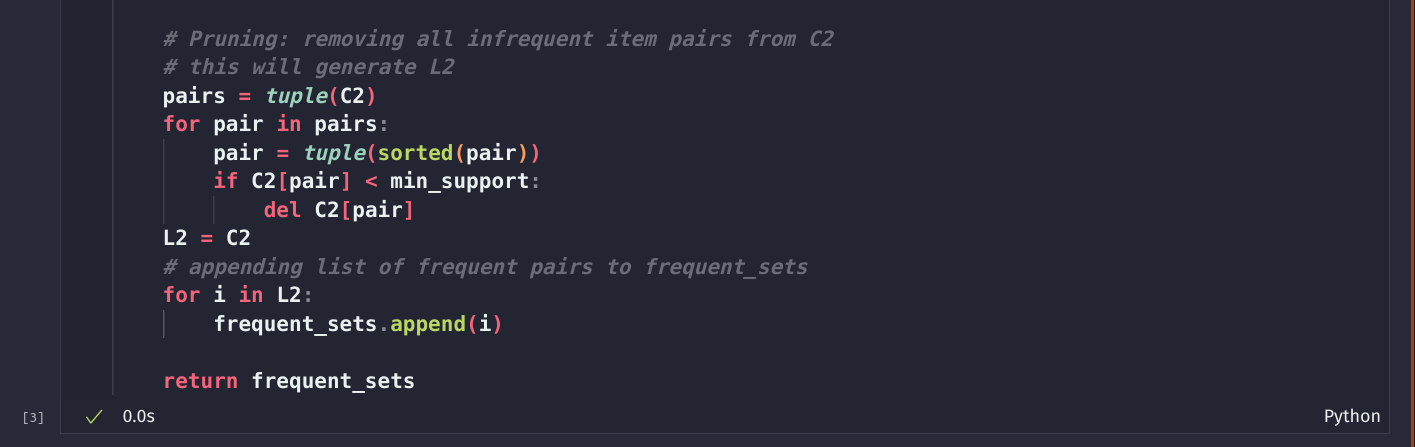
\includegraphics[width=1\textwidth, height=0.2\textheight]{./a.png}
            \end{figure}
        \end{minipage}

        \item \begin{minipage}[t]{0.9\textwidth}
            Downloading retail dataset for the PCY and Apriori algorithms:
            \begin{figure}[H]
                \centering
                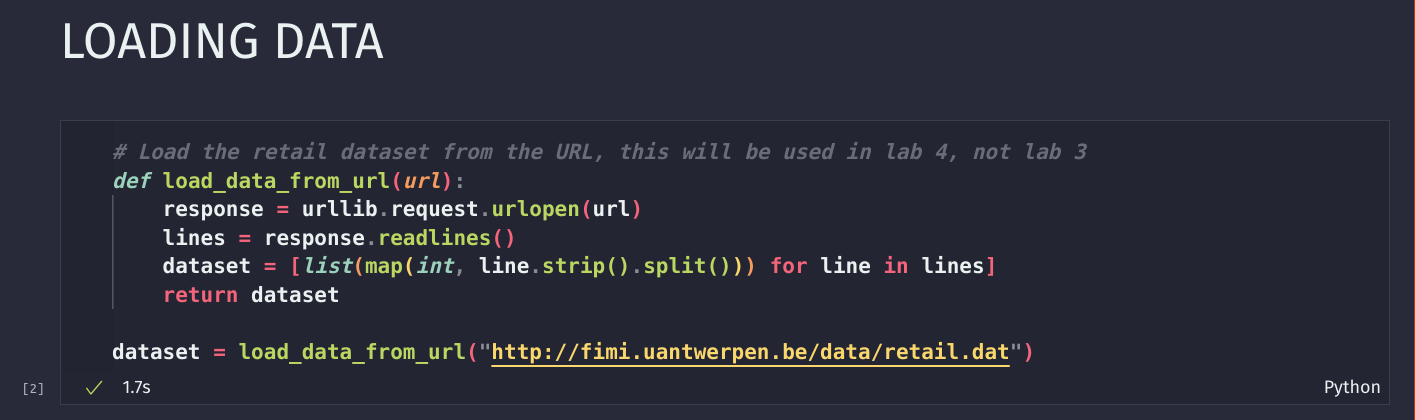
\includegraphics[width=1\textwidth, height=0.2\textheight]{./b.png}
            \end{figure}
        \end{minipage}
        
        \newpage

        \item \begin{minipage}[t]{0.9\textwidth}
            Comparing Apriori and PCY algorithms using the provided partitions
            of the dataset:
            \begin{figure}[H]
                \centering
                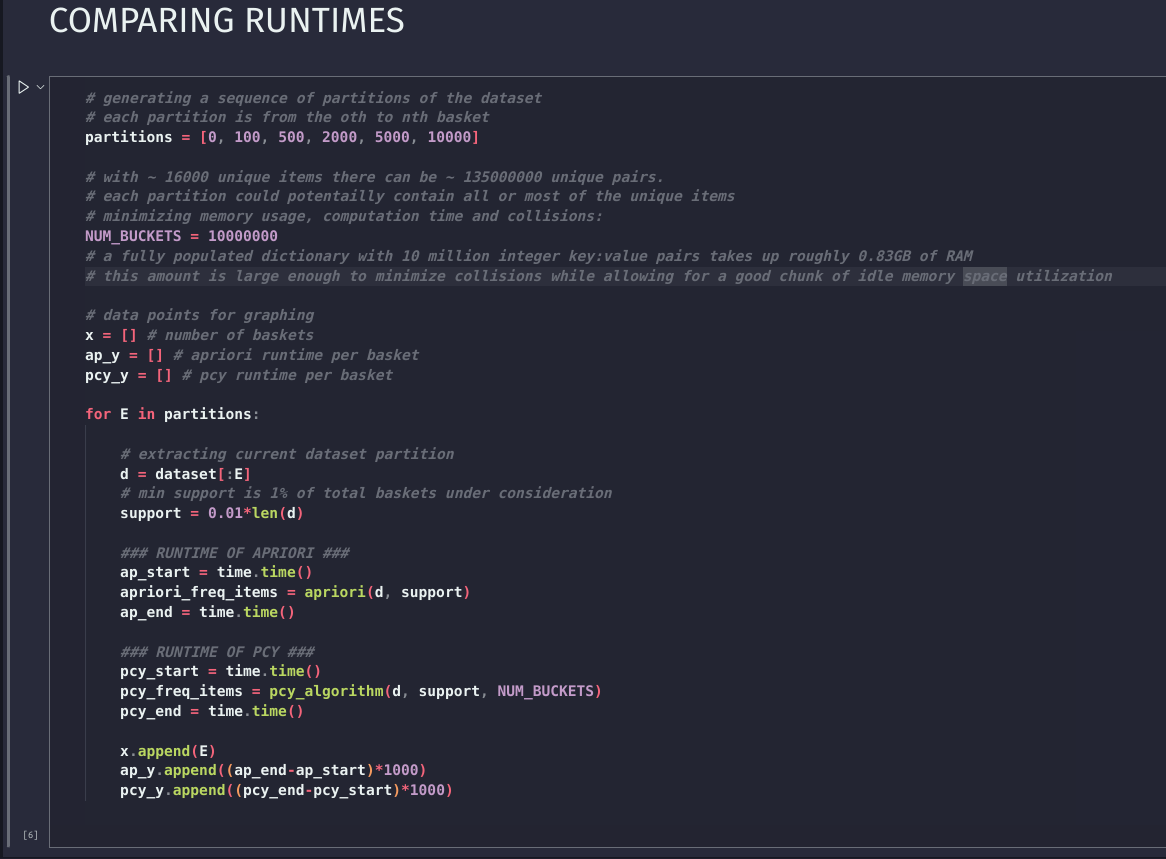
\includegraphics[width=1\textwidth, height=0.4\textheight]{./c.png}
            \end{figure}
        \end{minipage}

        \item \begin{minipage}[t]{0.9\textwidth}
            Graphing results. Dataset size is on the x-axis while runtime (ms) is on y-axis:
            \begin{figure}[H]
                \centering
                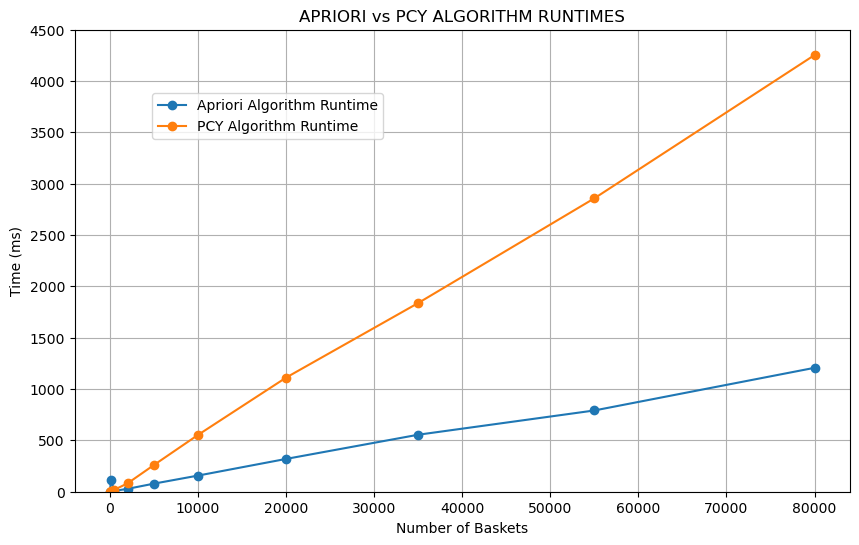
\includegraphics[width=1\textwidth, height=0.35\textheight]{./d.png}
            \end{figure}
        \end{minipage}

        \item \begin{minipage}[t]{0.9\textwidth}
            All screenshots have been provided.
        \end{minipage}
        
        \item \begin{minipage}[t]{0.9\textwidth}
            We can see that the PCY algorithm has a much faster runtime than Apriori which seems to increase exponentially
            faster as the datasets increase in size. This finding is consistent with expected performance results since 
            Apriori must generate and store all possible candidate pairs based on frequent singletons (which could be quite
            numerous, especially for low support values) while PCY generates candidate pairs based only on baskets
            encountered during a pass. Thus, PCY ends up generating far fewer pairs since the amount that actually
            exists in the dataset is usually much less than what is possible based on frequent singletons. 
        \end{minipage}

    \end{enumerate}

    \subsection*{Lab 5} 

    \begin{enumerate}[label=\alph*., left=10pt, itemsep=10pt]

        \item \begin{minipage}[t]{0.9\textwidth}
            The Jaccard similarity of two sets is the size of their intersection divided by the union.
            
            We have the following sets:
            \begin{align*}
                C_{1} &= \{2,3,4,5\}\\
                C_{2} &= \{3,4,6,8\}\\
                C_{3} &= \{2,3,6\}
            \end{align*}
            
            We can now calculate the Jaccard similarity of each pair of the above sets:
            \begin{align*}
                sim(C_{1},C_{2}) &= \frac{|C_{1} \cap C_{2}|}{|C_{1} \cup C_{2}|}\\
                                 &= \frac{|\{2,3,4,5\} \cap \{3,4,6,8\}|}{|\{2,3,4,5\} \cup \{3,4,6,8\}|}\\
                                 &= \frac{|\{3,4\}|}{|\{2,3,4,5,6,8\}|}\\
                                 &= \frac{2}{6}\\
                                 &= \frac{1}{3} = 0.3\overline{3}\\
                \\
                sim(C_{1},C_{3}) &= \frac{|C_{1} \cap C_{3}|}{|C_{1} \cup C_{3}|}\\
                                 &= \frac{|\{2,3,4,5\} \cap \{2,3,6\}|}{|\{2,3,4,5\} \cup \{2,3,6\}|}\\
                                 &= \frac{|\{2,3\}|}{|\{2,3,4,5,6\}|}\\
                                 &= \frac{2}{5} = 0.4\\
                \\
                sim(C_{2},C_{3}) &= \frac{|C_{2} \cap C_{3}|}{|C_{2} \cup C_{3}|}\\
                                 &= \frac{|\{3,4,6,8\} \cap \{2,3,6\}|}{|\{3,4,6,8\} \cup \{2,3,6\}|}\\
                                 &= \frac{|\{3,6\}|}{|\{2,3,4,6,8\}|}\\
                                 &= \frac{2}{5} = 0.4\\
            \end{align*}
        \end{minipage}
        \item \begin{minipage}[t]{0.9\textwidth}
            To find the expected value of the Jaccard similarity between sets $S$ and $T$ where $S, T \subseteq U$, $|S|=|T| = m$
            and $|U|= n$ we utilize the definition of expected value of functions of random variables:\\
            \begin{equation}
                \mathbb{E}(\phi(K)) = \sum\limits_{k \in \Omega} \phi(k)\cdot P(K=k)
            \end{equation}
            The above equation states that the expected value of a function of a random variable is the sum of the function evaluated
            for all possible inputs multiplied by the probability of said input.
            \\\\
            \textbf{First we find $\mathbf{\phi(k)}$.}\\\\
            Given that sets $S$ and $T$ are randomly selected subsets of $U$, we treat the cardinality of their intersection as a random
            variable and define their Jaccard similarity as a function of this random variable. We thus let $|S \cap T| = k$ and
            by the principle of inclusion-exclusion, note that $|S \cup T| = |S| + |T| - |S \cap T| = 2m - k$, giving us the following:
            \begin{equation}
                Sim(S,T) = \frac{|S \cap T|}{|S \cup T|} = \frac{k}{2m-k} = \phi(k)
            \end{equation}

            \textbf{Next we find $\mathbf{\mathbb{P}(K=k)}$.}\\\\
            Note that there are $\binom{n}{k}$ ways to select $k$ elements for our intersection. The remaining $m-k$ elements
            of either $S$ or $T$ can be selected in $\binom{n-k}{m-k}$ ways and the remaining $m-k$ elements of the final
            set can be chosen in $\binom{n-m}{m-k}$ ways. Thus, there are $\binom{n}{k} \cdot \binom{n-k}{m-k}
            \cdot \binom{n-m}{m-k}$ ways to choose $S$ and $T$ such that $|S \cap T| = k$.
            The number of ways to select an arbitrary set of length $m$ from $n$ total elements is $\binom{n}{m}$ meaning there
            are $\binom{n}{m}^{2}$ ways of selecting two consecutive subsets of $m$ elements from $n$ total.
            We thus define the probability of having $k$ elements in our intersection:
            \begin{equation}
                \mathbb{P}(K=k) = \frac{\binom{n}{k}\binom{n-k}{m-k}\binom{n-m}{m-k}}{\binom{n}{m}^{2}}
            \end{equation}

            A final observation is regarding our bounds of summation. We can have a maximum intersection of $k=m$ and a minimum
            intersection of $k = max(0, 2m-n)$ since sufficiently large subsets will make it impossible for them to be disjoint.\\\\
            
            \textbf{Defining $\mathbf{\mathbb{E}(Sim(S,T))}$.}\\\\
            We thus arrive at our final definition for expected Jaccard similarity:

            \begin{equation}
                \mathbb{E}(Sim(S,T)) = \mathbb{E}(\phi(K)) = \sum\limits_{k = max(0,2m-n)}^{m} \frac{k}{2m-k}\cdot \frac{\binom{n}{k}\binom{n-k}{m-k}\binom{n-m}{m-k}}{\binom{n}{m}^{2}}                
            \end{equation}
            
            \end{minipage}
            \newpage
            \begin{minipage}[t]{0.9\textwidth}
            Using simulations, we can demonstrate that the average Jaccard similarity over repeated trials converges to our
            calculated expected Jaccard similarity:
            \begin{figure}[H]
                \centering
                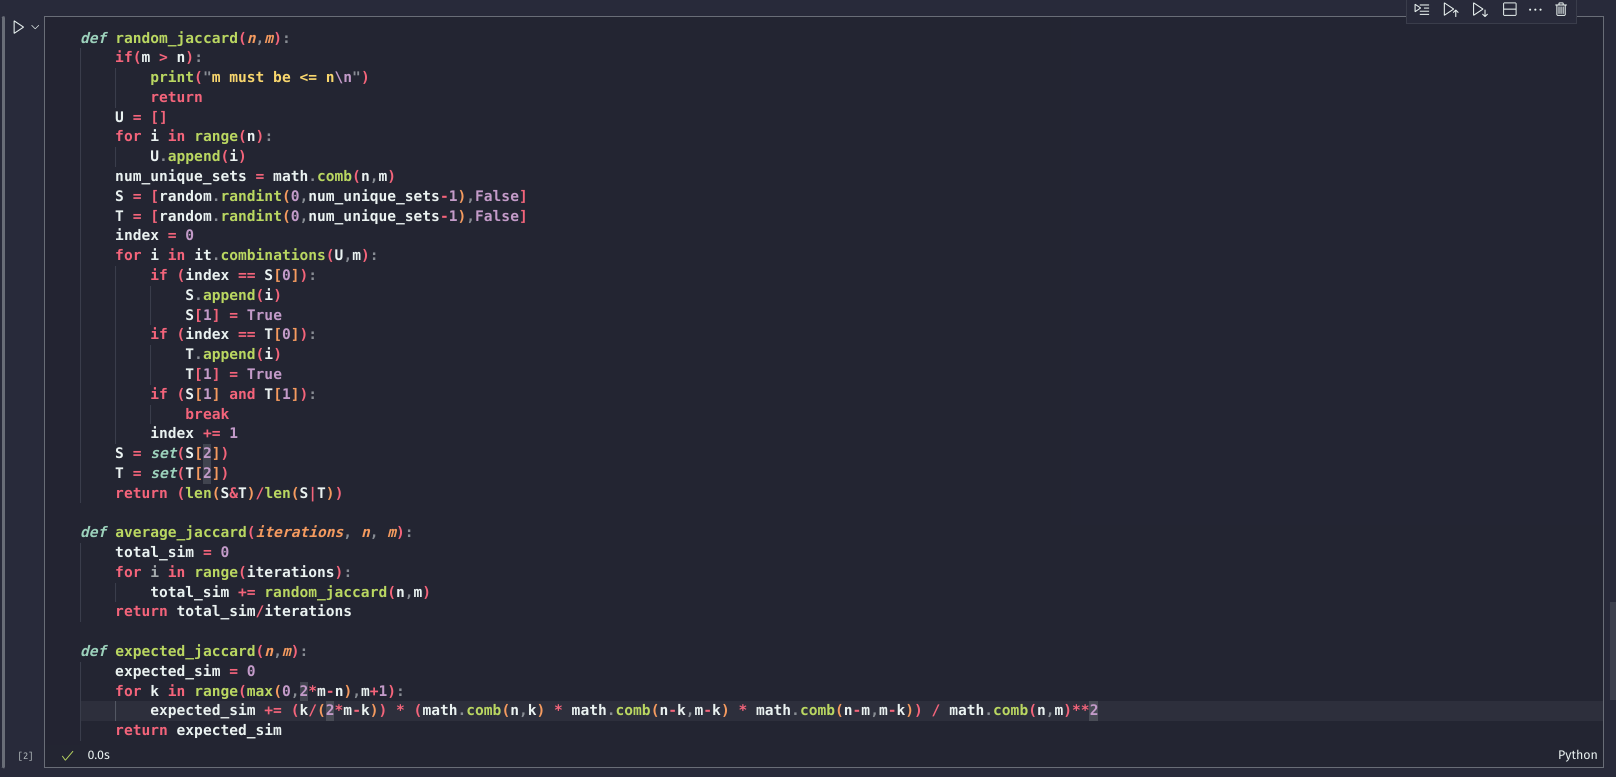
\includegraphics[width=1\textwidth, height=0.35\textheight]{./5bi.png}
                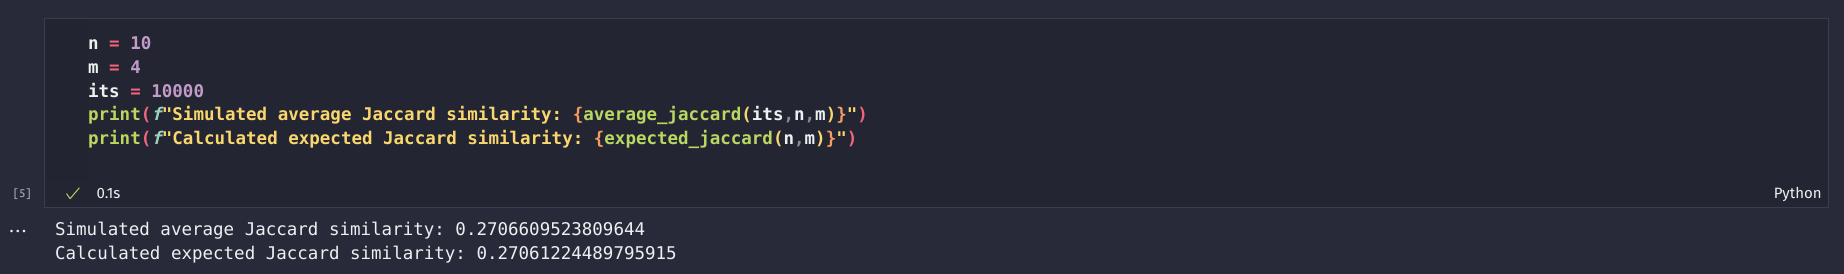
\includegraphics[width=1\textwidth, height=0.1\textheight]{./5bii.png}
            \end{figure}

        \end{minipage}

        \item \begin{minipage}[t]{0.9\textwidth}
            If we assume the number of possible strings of length $k$ is at least $n$, and we let $k=1$, then there must be $n$ unique 1-strings
            which implies there must be $n$ unique characters in our document and so all k-shingles must be unique.
            If we now imagine a k-shingle with $1 \leq k \leq n$ positioned such that the first character of the shingle is the first character of
            our document, we will be able to shift this shingle $n-k$ positions until the last character of the k-shingle is the last character of
            the document. Since every translation corresponds to a unique k-shingle we have shown there are at least $n-k$ total k-shingles. Finally,
            we add our initially positioned k-shingle to the count and conclude that there can be a maximum of $n-k+1$ k-shingles in a document of
            $n$ bytes.
        \end{minipage}

    \end{enumerate}

\end{document}